\documentclass[tikz,border=10pt]{standalone}
\usepackage{amsmath,amssymb}
\usetikzlibrary{arrows.meta,calc,positioning}

\begin{document}
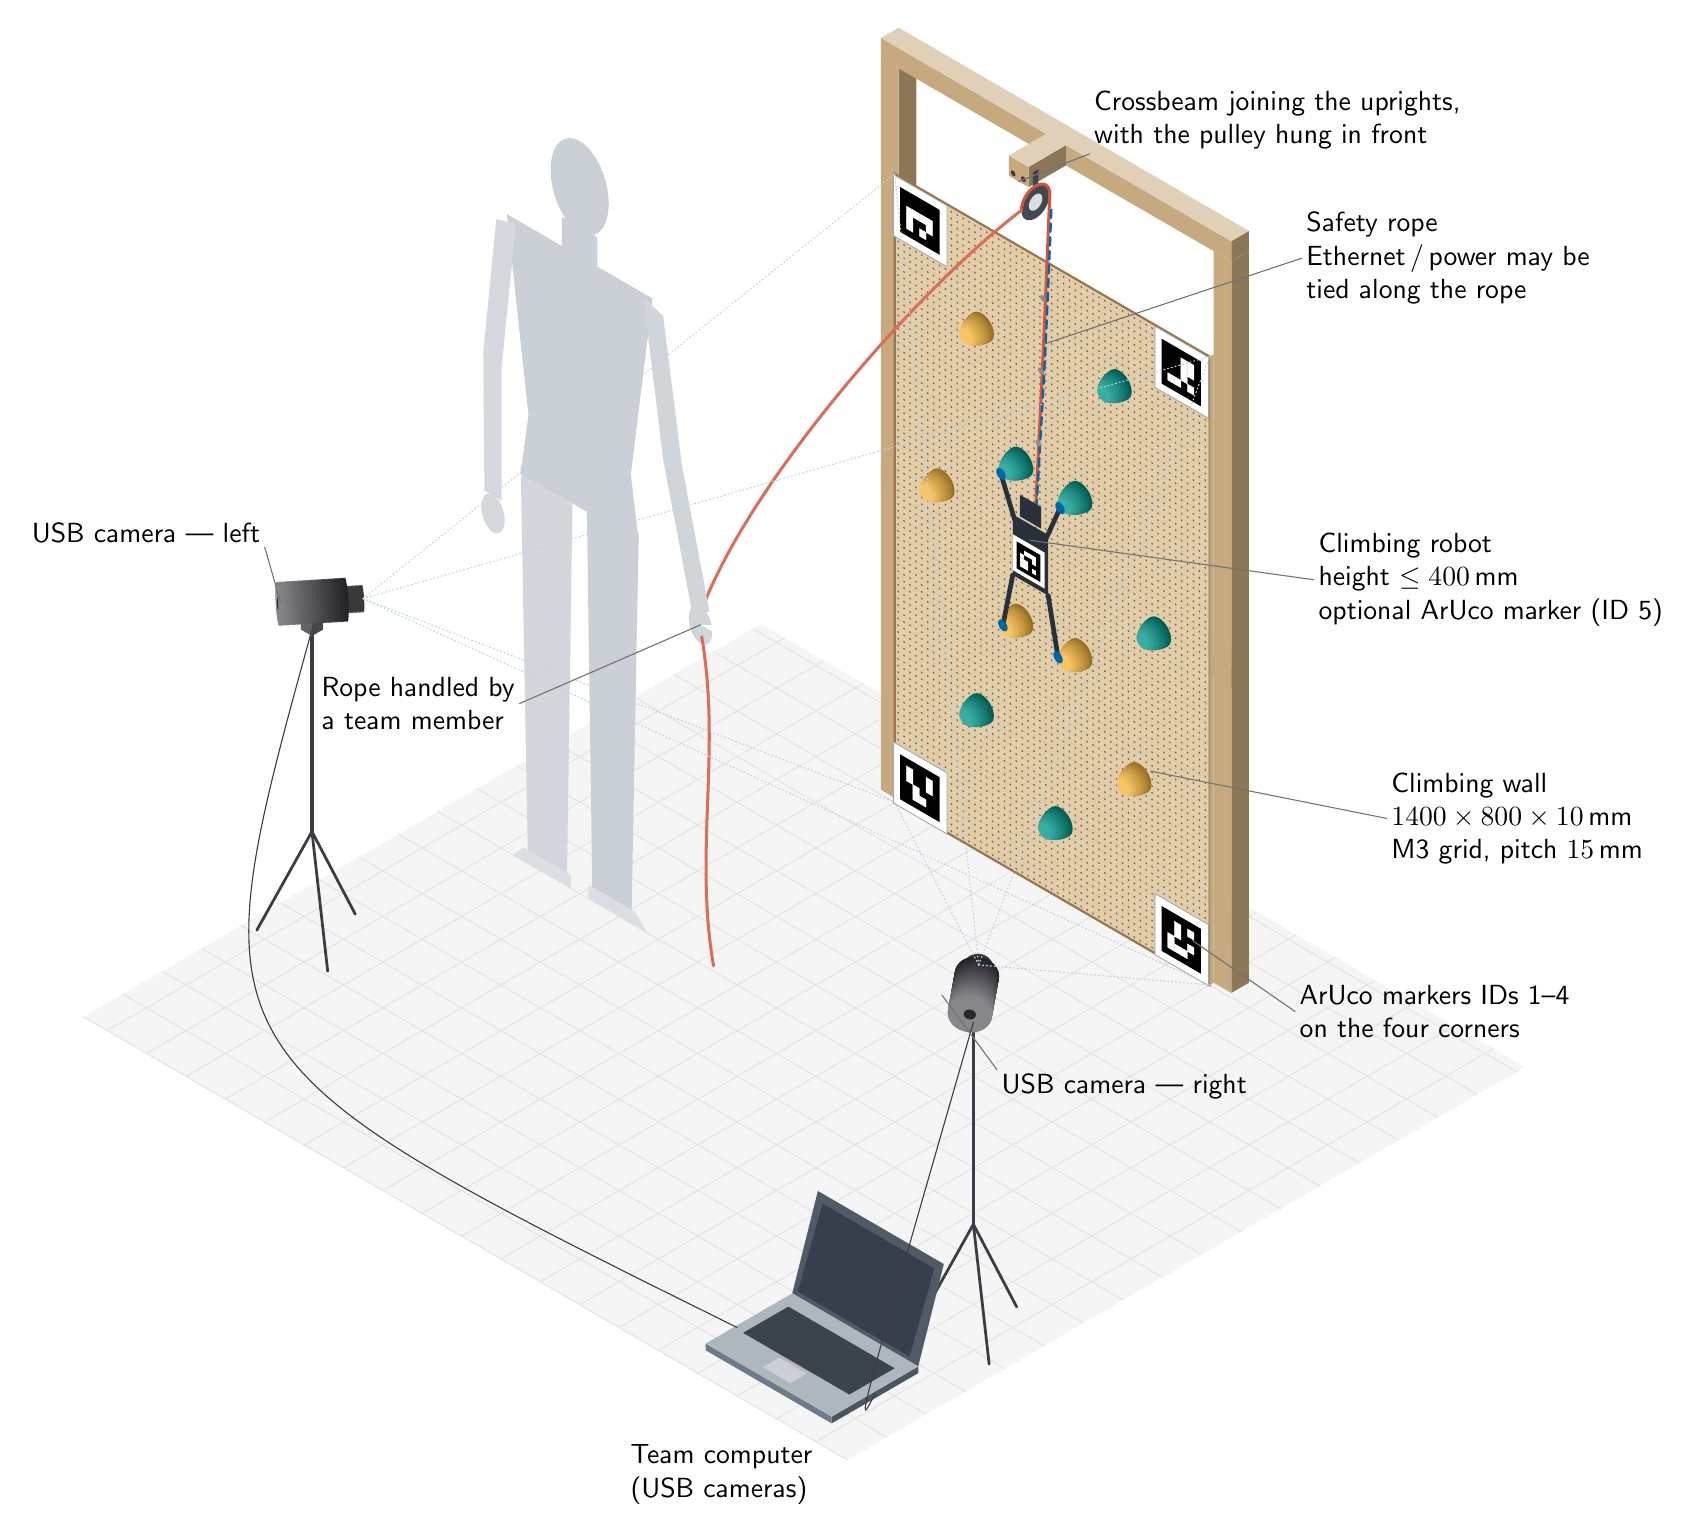
\begin{tikzpicture}[
    x={(0.50cm,-0.29cm)}, y={(0.50cm,0.29cm)}, z={(0cm,0.57cm)}, % 1 unit = 100 mm
    >={Stealth[length=5pt,width=4pt]},
    font=\sffamily\small,
    lead/.style={thin,black!55},
    lab/.style={font=\sffamily,align=left,inner sep=1.5pt},
    line cap=round,
  ]
  \definecolor{wood}{RGB}{226,205,171}
  \definecolor{woodE}{RGB}{150,120,80}
  \definecolor{woodD}{RGB}{198,169,126}
  \definecolor{steel}{RGB}{108,122,137}
  \definecolor{acc}{RGB}{0,102,170}
  \definecolor{rope}{RGB}{214,84,58}
  \definecolor{cam}{RGB}{60,60,68}
  \definecolor{bot}{RGB}{40,48,60}
  \definecolor{human}{RGB}{203,208,214}

  % isometric box: x y z dx dy dz color
  \newcommand{\isobox}[7]{%
    \fill[#7!70!black] ({#1+#4},#2,#3) -- ++(0,#5,0) -- ++(0,0,#6) -- ++(0,-#5,0) -- cycle;
    \fill[#7]          (#1,#2,#3) -- ++(#4,0,0) -- ++(0,0,#6) -- ++(-#4,0,0) -- cycle;
    \fill[#7!55!white] (#1,#2,{#3+#6}) -- ++(#4,0,0) -- ++(0,#5,0) -- ++(-#4,0,0) -- cycle;}

  % A disc lying in the wall plane (x,z) projects to a sheared ellipse spanned by
  % the x and z vectors. TikZ's "circle" uses the x and y vectors instead,
  % which lays the disc flat in the horizontal plane -- wrong for the holes, holds
  % and bolts that sit on the wall. Inside \wallplane the y vector is redefined
  % as the z vector, so a coordinate (u,v) means u*x+v*z and "circle" draws
  % the correct ellipse; the depth y is applied beforehand as a plain shift.
  \tikzset{wallplane/.style={y={(0cm,0.57cm)}}}
  % \wdisc{style}{x}{y}{z}{r}: filled disc of radius r in the wall plane, at depth y
  \newcommand{\wdisc}[5]{\begin{scope}[shift={(0,#3,0)}]\begin{scope}[wallplane]%
    \fill[#1] (#2,#4) circle (#5);\end{scope}\end{scope}}

  % ArUco markers on the wall: black code \AK + white border \AB (units of
  % 100 mm), outer corner of the border on the wall corner. Genuine
  % DICT_4X4_50 patterns (white cells), generated by gen_aruco.py.
  % GEN ARUCO BEGIN
  \def\arucoA{1/3,2/3,3/3,4/3,1/2,4/2,1/1,3/1}% ID 1
  \def\arucoB{3/4,4/4,3/3,4/3,3/2,1/1,2/1,4/1}% ID 2
  \def\arucoC{1/4,4/4,1/3,4/3,2/2,2/1,3/1}% ID 3
  \def\arucoD{2/4,4/4,2/3,1/2,4/2,1/1,2/1,3/1}% ID 4
  \def\arucoE{2/4,3/4,4/4,1/3,4/3,1/2,2/2,1/1,2/1,4/1}% ID 5
  % GEN ARUCO END
  \def\AK{1.0}\def\AB{0.18}\pgfmathsetmacro{\AT}{\AK+2*\AB}
  \newcommand{\arucoW}[3]{% x0 z0 (lower-left of the plate), white-cell list
    \fill[white,draw=black!35,line width=0.3pt]
      (#1,-0.03,#2) -- ++(\AT,0,0) -- ++(0,0,\AT) -- ++(-\AT,0,0) -- cycle;
    \fill[black] ({#1+\AB},-0.04,{#2+\AB}) -- ++(\AK,0,0) -- ++(0,0,\AK) -- ++(-\AK,0,0) -- cycle;
    \foreach \c/\r in #3{
      \filldraw[white,line width=0.1pt] ({#1+\AB+\AK*\c/6},-0.05,{#2+\AB+\AK*\r/6})
        -- ++(\AK/6,0,0) -- ++(0,0,\AK/6) -- ++(-\AK/6,0,0) -- cycle;}}

  %% ================= floor =================
  \fill[black!4] (-5.6,-15,0) -- (13.8,-15,0) -- (13.8,2.2,0) -- (-5.6,2.2,0) -- cycle;
  \foreach \i in {-5,-4,...,13}{\draw[black!10,thin] (\i,-15,0) -- (\i,2.2,0);}
  \foreach \j in {-15,-14,...,2}{\draw[black!10,thin] (-5.6,\j,0) -- (13.8,\j,0);}

  %% ================= wall support frame (behind) =================
  % The mid-height brace spans the whole frame, so its lit top face used to cut
  % across both posts and make them look severed. Drawing it first lets the two
  % posts paint over it and read as single uprights; the brace itself stays
  % hidden behind the wall panel, which is exactly where it sits.
  % Painter order runs from the far side to the near side. The viewer is on the
  % +x, -y side, so smaller x is further away: brace, then left upright, then
  % right upright. The crossbeam rests on top of both uprights and is drawn last,
  % which is also the only order that gets the joints right -- a crossbeam butted
  % between the uprights would have to be drawn after the left one and before the
  % right one, and its end grain would show.
  \isobox{-0.45}{0.1}{6.8}{8.9}{0.45}{0.45}{woodD}%  mid-height brace
  \isobox{-0.45}{0.1}{0}{0.45}{0.45}{16.3}{woodD}%   left upright
  \isobox{8.0}{0.1}{0}{0.45}{0.45}{16.3}{woodD}%     right upright
  \isobox{-0.45}{0.1}{16.3}{8.9}{0.45}{0.45}{woodD}% crossbeam, sitting on both

  %% ================= climbing wall =================
  \fill[wood,draw=woodE,thick] (0,0,0) -- (8,0,0) -- (8,0,14) -- (0,0,14) -- cycle;
  \fill[woodE!45!wood] (8,0,0) -- (8,0.10,0) -- (8,0.10,14) -- (8,0,14) -- cycle;
  \begin{scope}[shift={(0,-0.01,0)},wallplane]
    \foreach \i in {0,...,52}{\foreach \j in {0,...,92}{
        \fill[woodE!80!black] ({0.1+\i*0.15},{0.1+\j*0.15}) circle (0.024);}}
  \end{scope}

  \definecolor{holdA}{RGB}{0,150,136}\definecolor{holdB}{RGB}{247,181,56}
  % \hold{colour}{x}{z}: a jug seen in projection. Stacked wall-plane shells,
  % each one smaller, further out of the wall and lighter; because -y projects
  % down and to the left, the stack naturally leans that way and reads as a dome
  % rather than as a flat coloured disc.
  \newcommand{\hold}[3]{%
    \colorlet{hrim}{#1!62!black}\colorlet{htip}{#1!78!white}%
    \foreach \k in {0,...,8}{%
      \pgfmathsetmacro{\t}{\k/8}%
      \pgfmathsetmacro{\hr}{0.31*(1-0.45*\t*\t)}%
      \pgfmathsetmacro{\hy}{-0.04-0.40*\t}%
      \pgfmathsetmacro{\hm}{100-100*\t}%
      \wdisc{hrim!\hm!htip}{#2}{\hy}{#3}{\hr}}}
  \foreach \hx/\hz/\hc in {3.25/9.25/holdA, 4.75/9.25/holdA, 3.25/5.75/holdB,
      4.75/5.75/holdB, 2.25/3.25/holdA, 6.25/3.75/holdB, 1.25/7.75/holdB,
      6.75/7.25/holdA, 2.25/11.75/holdB, 5.75/12.25/holdA, 4.25/1.75/holdA}
     {\hold{\hc}{\hx}{\hz}}

  % ArUco markers at the four corners
  \arucoW{0}{14-\AT}{\arucoA} \arucoW{8-\AT}{14-\AT}{\arucoB}
  \arucoW{0}{0}{\arucoC}      \arucoW{8-\AT}{0}{\arucoD}

  %% ============ pulley, hung off the crossbeam over the top of the wall ========
  % A short bracket is cantilevered forward from the middle of the crossbeam so
  % that the pulley, and therefore both strands of the rope, hang clear of the
  % wall face. The wheel turns in a plane normal to the wall, i.e. x = 4.
  \isobox{3.75}{-0.85}{16.3}{0.5}{0.95}{0.45}{woodD}
  \wdisc{steel!50!black}{3.87}{-0.86}{16.42}{0.06}
  \wdisc{steel!50!black}{4.13}{-0.86}{16.42}{0.06}
  \fill[steel!55!black] (4.0,-0.49,16.32) -- (4.0,-0.35,16.32)
                      -- (4.0,-0.35,15.62) -- (4.0,-0.49,15.62) -- cycle;% hanger
  \fill[steel!60!black] plot[domain=0:360,samples=37,smooth] (4.0,{-0.42+0.36*cos(\x)},{15.62+0.36*sin(\x)});
  \fill[steel!25!white] plot[domain=0:360,samples=37,smooth] (4.0,{-0.42+0.17*cos(\x)},{15.62+0.17*sin(\x)});
  \coordinate (Ppulley) at (4.0,-0.85,16.30);

  %% ================= rope + tether (drawn behind the robot) ==========
  % rope over the top of the wheel, then down each vertical tangent
  \draw[rope,line width=1.1pt] plot[domain=0:180,samples=25,smooth]
        (4.0,{-0.42+0.36*cos(\x)},{15.62+0.36*sin(\x)});
  \draw[rope,line width=1.1pt] (4.00,-0.06,15.62) .. controls (4.0,-0.20,12.6) .. (4.00,-0.43,8.60);
  \draw[acc,line width=0.85pt,densely dashed]
        (4.10,-0.12,15.35) .. controls (4.14,-0.3,12.4) .. (4.12,-0.55,8.45);
  % cable ties along the rope, from (4.02,-0.18,15.3) to (4.05,-0.45,9.0)
  \foreach \t in {0.3,0.55,0.8}
     {\wdisc{black!45}{4.02+\t*0.03}{-0.18-\t*0.27}{15.3-\t*6.3}{0.07}}
  \coordinate (Prope) at (4.04,-0.3,12.4);

  %% ================= robot =================
  \begin{scope}[shift={(3.25,-0.55,5.75)}]
    \draw[bot,line width=1.7pt] (0.30,0,1.40) -- (0.05,0,0.15);
    \draw[bot,line width=1.7pt] (1.20,0,1.40) -- (1.45,0,0.15);
    \fill[bot] (0.30,0,1.40) -- (1.20,0,1.40) -- (1.20,0,2.75) -- (0.30,0,2.75) -- cycle;
    \fill[bot] (0.48,0,2.80) -- (1.02,0,2.80) -- (1.02,0,3.28) -- (0.48,0,3.28) -- cycle;
    % optional ArUco marker on the robot (ID 5)
    \fill[white] (0.35,-0.04,1.55) -- ++(0.80,0,0) -- ++(0,0,0.80) -- ++(-0.80,0,0) -- cycle;
    \fill[black] (0.45,-0.05,1.65) -- ++(0.60,0,0) -- ++(0,0,0.60) -- ++(-0.60,0,0) -- cycle;
    \foreach \c/\r in \arucoE{
      \fill[white] ({0.45+0.1*\c},-0.06,{1.65+0.1*\r})
        -- ++(0.1,0,0) -- ++(0,0,0.1) -- ++(-0.1,0,0) -- cycle;}
    \draw[bot,line width=1.7pt] (0.35,0,2.65) -- (0.00,0,3.50);
    \draw[bot,line width=1.7pt] (1.15,0,2.65) -- (1.50,0,3.50);
    \begin{scope}[wallplane]
      \fill[acc] (0,3.50) circle (0.12) (1.5,3.50) circle (0.12);
      \fill[acc] (0.05,0.15) circle (0.12) (1.45,0.15) circle (0.12);
    \end{scope}
    \coordinate (Pbot)   at (0.75,0,2.4);
    \coordinate (Parbot) at (0.75,0,1.60);
  \end{scope}

  %% ================= free rope end + team member =================
  \def\PX{-2.0}\def\PY{-6.0}
  \draw[rope!85,line width=1.1pt]
       (4.00,-0.78,15.62) .. controls (3.2,-2.6,14.4) and (1.2,-5.0,10.2)
       .. ({\PX+3.05},\PY,7.75);
  \begin{scope}[shift={(\PX,\PY,0)}]
    % legs
    \fill[human!85] (-1.50,0,8.80) -- (-0.18,0,8.80) -- (-0.32,0,0.30) -- (-1.32,0,0.30) -- cycle;
    \fill[human]    ( 1.50,0,8.80) -- ( 0.18,0,8.80) -- ( 0.32,0,0.30) -- ( 1.32,0,0.30) -- cycle;
    \fill[human!70] (-1.42,0,0.30) -- (-0.22,0,0.30) -- (-0.22,0,0.00) -- (-1.70,0,0.00) -- cycle;
    \fill[human!70] ( 1.42,0,0.30) -- ( 0.22,0,0.30) -- ( 0.22,0,0.00) -- ( 1.70,0,0.00) -- cycle;
    % torso
    \fill[human] (-1.85,0,14.20) -- (1.85,0,14.20) -- (1.30,0,10.00)
              -- (1.50,0,8.60) -- (-1.50,0,8.60) -- (-1.30,0,10.00) -- cycle;
    % arms (shoulder, elbow, wrist): right hand holds the rope, left arm hangs
    \fill[human!90] (1.62,0,14.10) -- (2.12,0,13.95) -- (2.60,0,10.85)
                 -- (3.30,0,7.95) -- (2.85,0,7.75) -- (2.12,0,10.75) -- cycle;
    \fill[human!90] (3.07,0,7.55)
      \foreach \a in {20,40,...,360} {-- ({3.07+0.30*cos(\a)},0,{7.55+0.42*sin(\a)})} -- cycle;
    \fill[human!80] (-1.62,0,14.10) -- (-2.12,0,13.95) -- (-2.45,0,10.80)
                 -- (-2.42,0,7.75) -- (-1.98,0,7.75) -- (-1.98,0,10.75) -- cycle;
    \fill[human!80] (-1.90,0,7.35)
      \foreach \a in {20,40,...,360} {-- ({-2.20+0.30*cos(\a)},0,{7.35+0.42*sin(\a)})} -- cycle;
    % neck + head
    \fill[human] (-0.45,0,14.00) -- (0.45,0,14.00) -- (0.45,0,14.85) -- (-0.45,0,14.85) -- cycle;
    \fill[human] (0.74,0,15.75)
      \foreach \a in {12,24,...,360} {-- ({0.74*cos(\a)},0,{15.75+1.02*sin(\a)})} -- cycle;
    \coordinate (Phand) at (3.07,0,7.55);
  \end{scope}
  \draw[rope!85,line width=1.1pt]
       ({\PX+3.10},\PY,7.30) .. controls ({\PX+3.6},\PY,5.0) and ({\PX+2.9},\PY,2.4)
       .. ({\PX+3.4},\PY,0.12);

  %% ================= cameras =================
  % \usbcam{x}{y}{ax}{ay}: a USB webcam on a small tripod, aimed along the
  % horizontal unit vector (ax,ay). Both cameras stand in front of the wall and
  % look back at it, so their axis projects nearly horizontally for the left one
  % but almost vertically for the right one. The body is therefore built as a
  % stack of discs along the axis, far end first: that silhouette stays right at
  % any inclination, whereas a lateral quad built from vertical offsets collapses
  % as soon as the axis projects steeply. Each disc lies in the plane spanned by
  % z and the horizontal normal (ay,-ax), hence the parametric plots.
  \newcommand{\usbcam}[4]{%
    \pgfmathsetmacro{\cH}{7.0}%          height of the tripod head
    \pgfmathsetmacro{\cZ}{\cH+0.52}%     barrel axis height
    \pgfmathsetmacro{\cR}{0.40}%          barrel radius
    \pgfmathsetmacro{\cL}{0.25}%          lens housing radius
    \pgfmathsetmacro{\cPx}{#4}\pgfmathsetmacro{\cPy}{-#3}% in-plane normal
    \colorlet{camF}{cam!55!black}\colorlet{camB}{cam!62!white}%
    % tripod and neck
    \draw[cam,line width=1.0pt] (#1,#2,2.4) -- ++(-0.9,-0.5,-2.4);
    \draw[cam,line width=1.0pt] (#1,#2,2.4) -- ++(0.9,-0.5,-2.4);
    \draw[cam,line width=1.0pt] (#1,#2,2.4) -- ++(0.0,1.1,-2.4);
    \draw[cam,line width=1.2pt] (#1,#2,2.4) -- (#1,#2,\cH);
    \isobox{#1-0.14}{#2-0.14}{\cH-0.10}{0.28}{0.28}{0.50}{cam!80!white}
    % lens housing, the far end of the camera
    \foreach \k in {0,...,24}{%
      \pgfmathsetmacro{\cD}{0.92-0.35*\k/24}%
      \fill[black!78] plot[domain=0:360,samples=25,smooth]
        ({#1+\cD*#3+\cL*\cPx*cos(\x)},{#2+\cD*#4+\cL*\cPy*cos(\x)},{\cZ+\cL*sin(\x)});}
    % barrel, drawn from the lens end back to the rear cap
    \foreach \k in {0,...,80}{%
      \pgfmathsetmacro{\cD}{0.62-1.24*\k/80}%
      \pgfmathsetmacro{\cM}{100-1.25*\k}%
      \fill[camF!\cM!camB] plot[domain=0:360,samples=29,smooth]
        ({#1+\cD*#3+\cR*\cPx*cos(\x)},{#2+\cD*#4+\cR*\cPy*cos(\x)},{\cZ+\cR*sin(\x)});}
    % cable grommet on the rear cap
    \fill[cam!65!black] plot[domain=0:360,samples=21,smooth]
      ({#1-0.62*#3+0.11*\cPx*cos(\x)},{#2-0.62*#4+0.11*\cPy*cos(\x)},{\cZ+0.11*sin(\x)});}
  \usbcam{-4.4}{-10.4}{0.628}{0.778}
  \usbcam{12.6}{-10.6}{-0.630}{0.777}
  \coordinate (PcamL) at (-4.85,-10.75,7.46);
  \coordinate (PcamR) at (12.15,-10.95,7.46);

  % Sight lines leave the front of each lens housing -- the camera centre plus
  % 0.92 along its aim axis, at the barrel axis height 7.52 -- rather than the
  % middle of the body, so they visibly come out of the objective.
  \foreach \cx/\cy in {-3.822/-9.684, 12.020/-9.885}{
    \foreach \wx/\wz in {0/14, 8/14, 0/0, 8/0}
      \draw[acc!28,thin,densely dotted] (\cx,\cy,7.52) -- (\wx,0,\wz);}

  %% ================= host PC: laptop =================
  % The lid hinges on the far edge of the base and leans away from the operator,
  % who stands on the -y side; its normal therefore points at the viewer. Drawn
  % before the base so the base overlaps it at the hinge.
  \fill[steel!75!black] (9.6,-12.2,0.15) -- (12.8,-12.2,0.15)
                     -- (12.8,-11.55,2.10) -- (9.6,-11.55,2.10) -- cycle;
  \fill[cam!92!acc]     (9.78,-12.24,0.30) -- (12.62,-12.24,0.30)
                     -- (12.62,-11.61,1.94) -- (9.78,-11.61,1.94) -- cycle;
  \isobox{9.6}{-14.4}{0}{3.2}{2.2}{0.15}{steel}
  % keyboard well and trackpad on the top face
  \fill[steel!55!black] (9.85,-13.70,0.16) -- ++(2.7,0,0) -- ++(0,1.15,0) -- ++(-2.7,0,0) -- cycle;
  \fill[steel!35!white] (10.85,-14.20,0.16) -- ++(0.7,0,0) -- ++(0,0.42,0) -- ++(-0.7,0,0) -- cycle;
  \coordinate (Ppc) at (11.2,-13.4,0.15);
  \draw[cam,thin] (-4.4,-10.4,6.9) .. controls (-3.0,-14.8,0.3) .. (9.6,-13.6,0.10);
  \draw[cam,thin] (12.6,-10.6,6.9) .. controls (13.6,-14.6,0.3) .. (12.8,-13.3,0.10);

  %% ================= annotations =================
  \node[lab,anchor=south west] (Lpul) at ($(Ppulley)+(0.9cm,0.35cm)$)
        {Crossbeam joining the uprights,\\ with the pulley hung in front};
  \draw[lead] (Lpul.south west) -- (Ppulley);

  \node[lab,anchor=west] (Lrope) at ($(Prope)+(3.3cm,1.1cm)$)
        {Safety rope\\ Ethernet\,/\,power may be\\ tied along the rope};
  \draw[lead] (Lrope.west) -- (Prope);

  \node[lab,anchor=west] (Lbot) at ($(Pbot)+(3.6cm,-0.5cm)$)
        {Climbing robot\\ height $\le 400$\,mm\\ optional ArUco marker (ID 5)};
  \draw[lead] (Lbot.west) -- (Pbot);

  \node[lab,anchor=west] (Lwall) at ($(6.5,0,4.0)+(3.0cm,-0.6cm)$)
        {Climbing wall\\ $1400\times800\times10$\,mm\\ M3 grid, pitch $15$\,mm};
  \draw[lead] (Lwall.west) -- (6.5,0,4.0);

  \node[lab,anchor=west] (Lar) at ($(7.6,-0.03,0.8)+(1.3cm,-0.9cm)$)
        {ArUco markers IDs 1--4\\ on the four corners};
  \draw[lead] (Lar.west) -- (7.6,-0.03,0.8);

  \node[lab,anchor=east] (Lper) at ($(Phand)+(-2.3cm,-1.0cm)$)
        {Rope handled by\\ a team member};
  \draw[lead] (Lper.east) -- (Phand);

  \node[lab,anchor=south east] (LcamL) at ($(PcamL)+(-0.2cm,0.7cm)$)
        {USB camera --- left};
  \draw[lead] (LcamL.south east) -- (PcamL);

  \node[lab,anchor=north west] (LcamR) at ($(PcamR)+(0.7cm,-0.95cm)$)
        {USB camera --- right};
  \draw[lead] (LcamR.north west) -- (PcamR);

  \node[lab,anchor=north] at ($(Ppc)+(-1.1cm,-1.05cm)$) {Team computer\\ (USB cameras)};
\end{tikzpicture}
\end{document}
